\section{Results}

To analyze the measured data, the Python \cite{python} packages NumPy \cite{numpy} and SciPy \cite{scipy} are used, with Matplotlib
\cite{matplotlib} generating the graphical presentation and Uncertainties \cite{uncertainties} allowing for automated linear order
propagation of errors.


\subsection{Verifying the Stability Condition}
As shown in \autoref{fig:stability} the stability condition for the used mirrors is fulfilled for different resonator lengths $L$. In the case of one planar mirror ($R_1=\infty$) and one out coupling mirror with radius $R_2=1400\, \unit{\nano \meter}$ the stability condition is true for 
a resonator length of up to $1.4\, \unit{\meter}$. Thus one would expect to see the laser working fine for smaller resonators. Analogously for a high reflective mirror ($R_1=1400\, \unit{\nano \meter}$) instead of the planar surface one find a maximum length of $L\leq 2.8\, \unit{\meter}$.
\begin{figure}
	\centering
	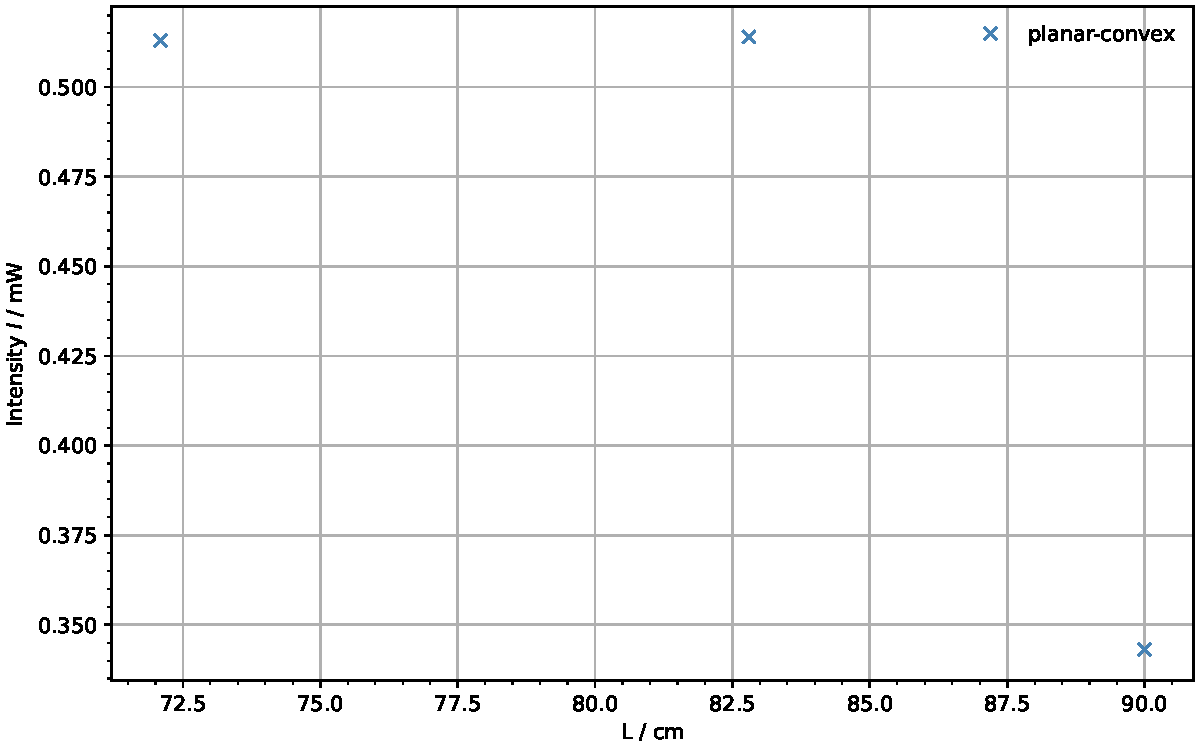
\includegraphics[width=0.8\textwidth]{content/plots/stability2.pdf}
	\caption{Measured Intensity in dependency of resonator length $L$ to verify the Stability Condition for one planar and one convex mirror.}
	\label{fig:stability2}
\end{figure}
\begin{figure}
	\centering
	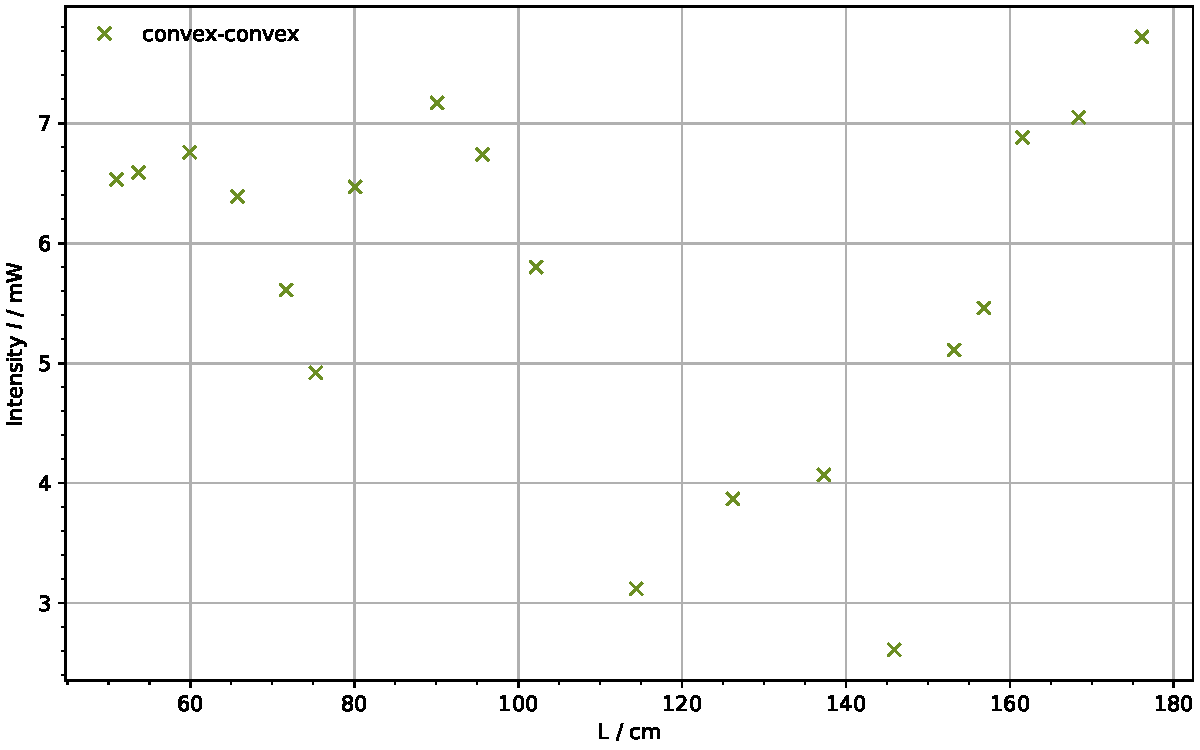
\includegraphics[width=0.8\textwidth]{content/plots/stability1.pdf}
	\caption{Measured Intensity in dependency of resonator length $L$ to verify the Stability Condition for two convex mirrors.}
	\label{fig:stability1}
\end{figure}
The measured intensities for different resonator lengths are displayed in \autoref{fig:stability2} and \autoref{fig:stability1}. One can see that the intensities are $\ll 0$ and therefore a stable operation of the laser is possible.

\subsection{Observing Transverse Modes}

The measured intensities for different deviations of the detector in $x$ directions are shown in \autoref{fig:TEM00}, \autoref{fig:TEM01} and \autoref{fig:TEM02}. The respective curve-fits follow the equations shown in \eqref{eqn:TEMEQN1}, \eqref{eqn:TEMEQN2}, \eqref{eqn:TEMEQN3}. Since the measurements are not exactly as 
predicted, the actual equations need to be adjusted.

\subsubsection{$\text{TEM}_{00}$}

For the $\text{TEM}_{00}$ follows 
\begin{equation*}
    I_{\text{fit,TEM}_{00}}(x) = I_{00} \cdot e^{-\frac{2 (x - m)^2}{w_0^2}}\; .
\end{equation*}
The definition of a new centre of the curve $m$ is necessary because the detector's deviation scale is not symmetrical around the beam's axis.
\begin{figure}
	\centering
	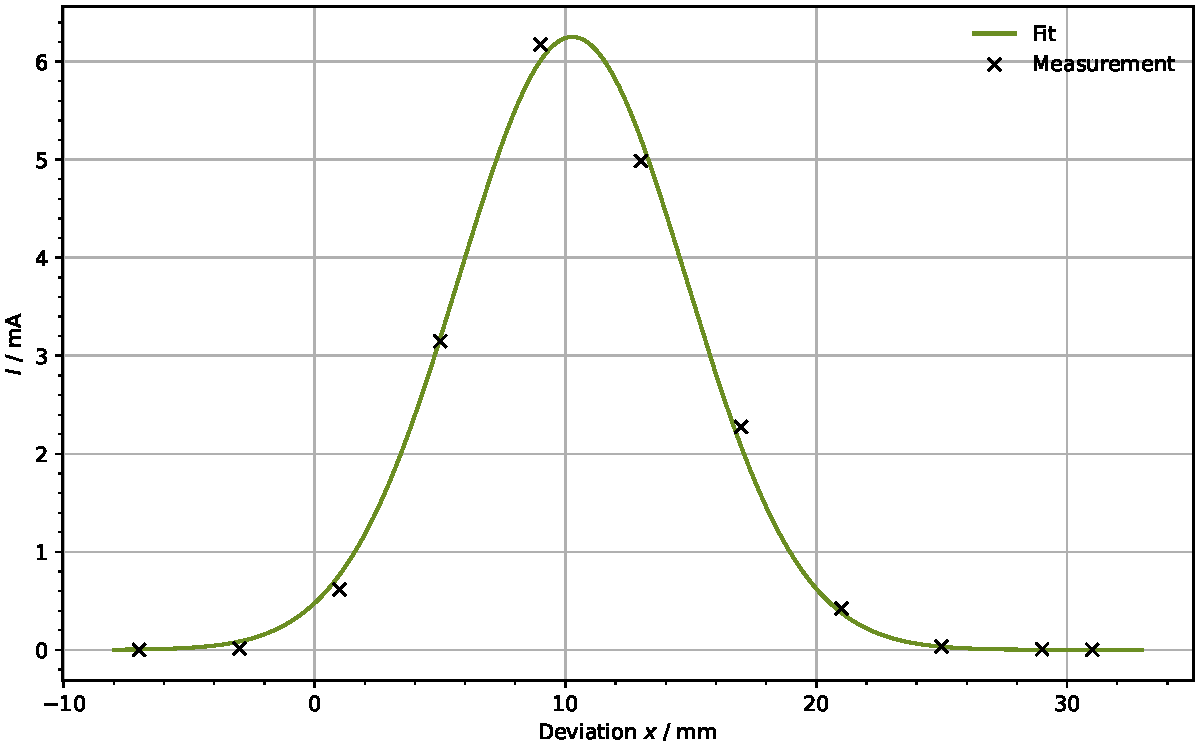
\includegraphics[width=0.8\textwidth]{content/plots/TEM00.pdf}
	\caption{Measured Intensity in dependency of the detectors $x$-position for observing $\text{TEM}_{00}$.}
	\label{fig:TEM00}
\end{figure}
The parameters for the fit are given by
\begin{align*}
    I_{00} &= (6.253\pm 0.118) \, \unit{\milli \watt}\\
    m &= (10.276\pm 0.099)\, \unit{\milli \meter}\\
    w_0 &= (9.058\pm 0.198) \, \unit{\milli \meter}\; .
\end{align*}

\subsubsection{$\text{TEM}_{10}$}

Analogously to the adjustment for intensity of $\text{TEM}_{00}$ the new fit curve can be determined to 
\begin{equation*}
    I_{\text{fit,TEM}_{10}}(x) = I_{10} \cdot \left( \frac{x - l}{w_0} \right)^2 \cdot e^{-\frac{2(x - m)^2}{w_0^2}}\; .
\end{equation*}
The newly introduced parameter $l$ is needed to describe the asymmetrical properties of the data.
\begin{figure}
	\centering
	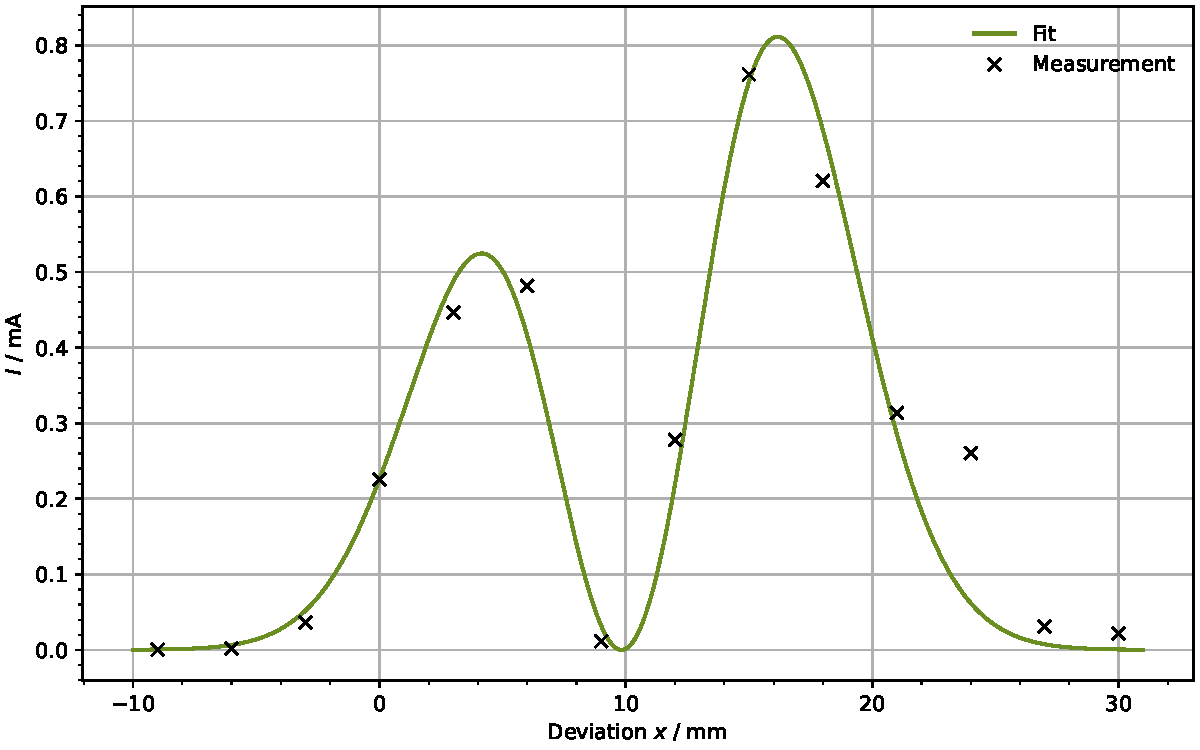
\includegraphics[width=0.8\textwidth]{content/plots/TEM01.pdf}
	\caption{Measured Intensity in dependency of the detectors $x$-position for observing $\text{TEM}_{10}$.}
	\label{fig:TEM01}
\end{figure}
For the new defined equation the parameters can be determined to 
\begin{align*}
I_{10} &= \left( 3.568 \pm 0.236 \right) \, \text{mW} \\
m &= \left( 10.483 \pm 0.264 \right) \, \text{mm} \\
w_0 &= \left( 8.480 \pm 0.335 \right) \, \text{mm} \\
l &= \left( 9.830 \pm 0.262 \right) \, \text{mm}
\end{align*}

\subsubsection{$\text{TEM}_{20}$}
The proper fit function can be defined by 

\begin{equation*}
    I_{\text{fit,TEM}_{20}}(x)  = I_{20} \cdot \left( 4 \left( \frac{x - l}{w_0} \right)^2 - 1 \right)^2 \cdot e^{-\frac{2(x - m)^2}{w_0^2}}\; .
\end{equation*}

\begin{figure}
	\centering
	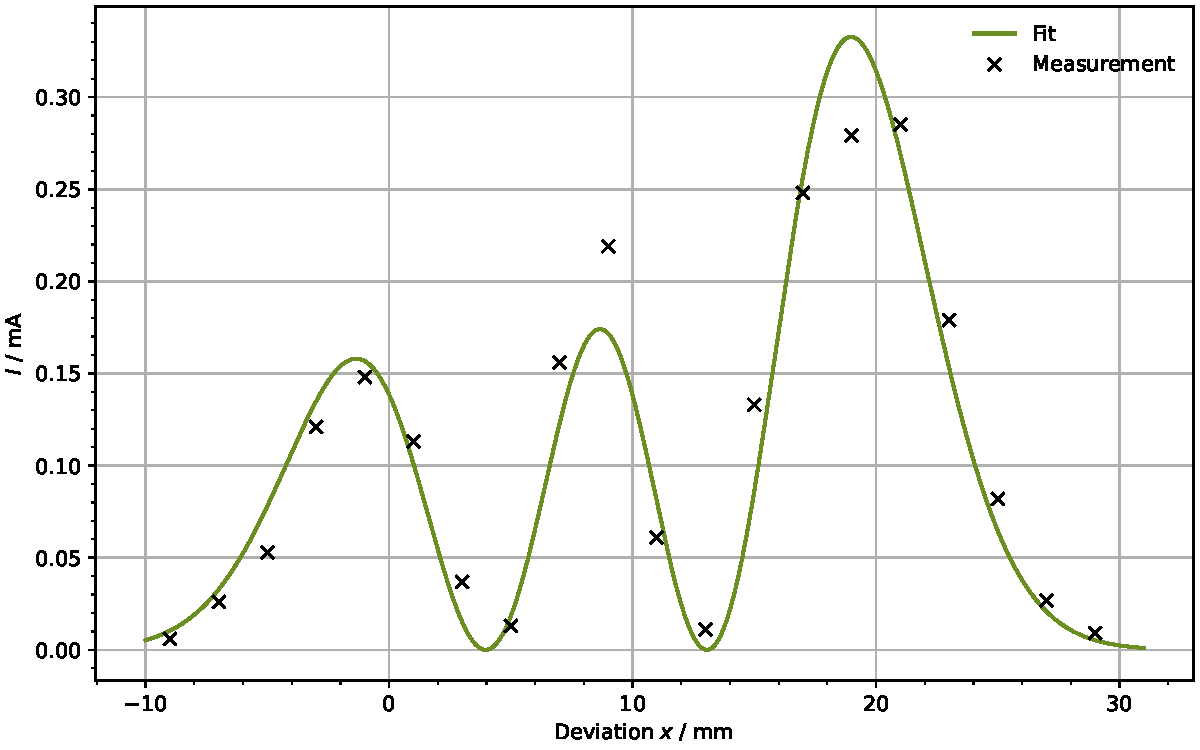
\includegraphics[width=0.8\textwidth]{content/plots/TEM02.pdf}
	\caption{Measured Intensity in dependency of the detectors $x$-position for observing $\text{TEM}_{20}$.}
	\label{fig:TEM02}
\end{figure}
The parameters are
\begin{align*}
    I_{20} &= \left( 0.176\pm0.009 \right) \, \text{mW} \\
    m &= \left( 9.266\pm0.190 \right) \, \text{mm} \\
    w_0 &= \left( 9.082\pm0.184 \right) \, \text{mm} \\
    l &= \left( 8.511\pm0.181 \right) \, \text{mm}
\end{align*}

\subsection{Determining the Polarization}

In order to determine the polarization of the laser, the measured intensities are plotted against the polarization filter's angle.
The general dependency of angle and intensity is given via \eqref{eqn:pol}. But similar to the chapters above, the equation needs to be slightly adjusted.
The final form is
\begin{equation*}
    I=I_0\cos(\phi-\alpha)^2+c\; .
\end{equation*}
The introduced parameter $c$ is needed to compensate any offset and $\alpha$ is used to compensate possible rotation that is occurs due to different orientations of the polarization direction.
\begin{figure}
	\centering
	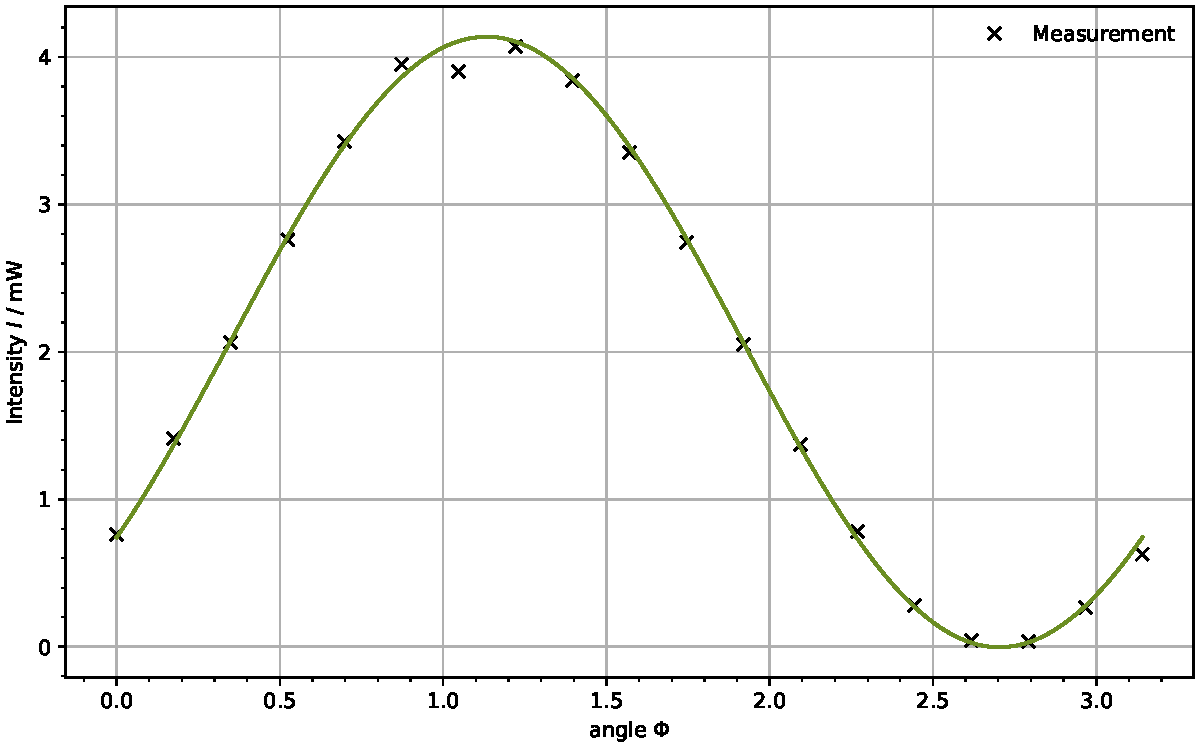
\includegraphics[width=0.8\textwidth]{content/plots/POLARI.pdf}
	\caption{Measured Intensity in dependency of the polarization filter's angle.}
	\label{fig:POLARI}
\end{figure}
The parameters are
\begin{align*}
    I_0 &= (4.140\pm 0.032) \, \text{mW}\\
\alpha &= 1.133\pm 0.004\\
c &= (-0.003\pm 0.018)\, \text{mW}\; .
\end{align*}

\subsection{Analyzing Spectra in Multimode Operation}

The experimental data for frequency and amplitude are shown in \autoref{tab:MULTI} with the resonator length.

\begin{table}[h!]
\centering
\caption{Experimental data after the FFT.}
\noindent\makebox[\linewidth]{
\begin{tabular}{|c|c|c|c|c|c|c|c|c|c|c|}
\hline
L in cm & \makecell{$f_1$ \\(MHz)} & \makecell{$\text{Ampl}_1$ \\(mV)} & \makecell{$f_2$ \\(MHz)} & \makecell{$\text{Ampl}_2$ \\(mV)} & \makecell{$f_3$ \\(MHz)} & \makecell{$\text{Ampl}_3$ \\(mV)} & \makecell{$f_4$ \\(MHz)} & \makecell{$\text{Ampl}_4$ \\(mV)} & \makecell{$f_5$ \\(MHz)} & \makecell{$\text{Ampl}_5$ \\(mV)} \\
\hline
53.7 & 279 & 958 & 560 & 870 & 836 & 740 & 1117 & 140 & 1393 & 80 \\
65.8 & 228 & 988 & 457 & 873 & 682 & 880 & 911 & 480 & 1141 & 160 \\
75.3 & 200 & 992 & 398 & 931 & 599 & 830 & 797 & 700 & 994 & 220 \\
90.1 & 169 & 1000 & 335 & 950 & 501 & 896 & 667 & 905 & 832 & 800 \\
\hline
\end{tabular}
}
\label{tab:MULTI}
\end{table}
In order to investigate the dependence of the resonator length and the measured frequencies one needs to calculate the $\Delta f$ between the peaks.

\begin{table}[h!]
    \centering
    \caption{Calculated differences between peak frequencies.}
	\noindent\makebox[\linewidth]{
    \begin{tabular}{|c|c|c|c|c|c|}
    \hline
    L in cm & $\Delta f_{1,2}$ / MHz &$\Delta f_{2,3}$ / MHz & $ \Delta f_{3,4}$ / MHz  & $\Delta f_{4,5}$ / MHz & avg. $\Delta f$ / MHz \\  
    \hline
    53.7 & 281.0 & 276.0 & 281.0 & 276.0 & 278.50\\
    65.8 & 229.0 & 225.0 & 229.0 & 230.0 & 228.25 \\
    75.3 & 198.0 & 201.0 & 198.0 & 197.0 & 198.50\\
    90.1 & 166.0 & 166.0 & 166.0 & 165.0 & 165.75 \\
    \hline
    \end{tabular}
	}
    \label{tab:diffF}
\end{table}
By solving \eqref{eqn:bla} for $L$ one can obtain the following resonator lengths 
\begin{align*}
    	\Delta f &= 278.50\, \text{MHz} \rightarrow 53.8\, \text{cm}\\
        \Delta f &= 228.25\, \text{MHz} \rightarrow 65.7\, \text{cm}\\
        \Delta f &= 198.50\, \text{MHz} \rightarrow 75.6\, \text{cm}\\
        \Delta f &= 165.75\, \text{MHz} \rightarrow 90.5\, \text{cm}\; .
\end{align*}

A different approach to clarify the dependence of resonator length and the distance between the spectral peaks is the graphical one shown in \autoref{fig:Resonlänge}. The fit for the data is calculated with 
\begin{equation*}
    \Delta f(L)=a\cdot L^{b}
\end{equation*}
with $a$ having the theoretical value of $a=c/2$ and $b=-1$ as one can obtain from \autoref{fig:Resonlänge}.
\begin{figure}[h!]
    \centering
    \includegraphics[width=0.8\textwidth]{content/plots/Resonlänge.pdf}
    \caption{Dependence of resonator length and distance between spectral peaks.}
    \label{fig:Resonlänge}
\end{figure}
The fit parameters are given by 
\begin{align*}
    a&= (147.1 \pm 0.1) 10^8\, \frac{\text{m}}{\text{s}} \\
    b&= -0.983 \pm 0.004\; .
\end{align*}

Further it is possible to measure and visualize the Doppler broadening described in \autoref{sec:doppler}. For doing so one additional measurement was performed with a larger resonator. Due to the larger resonator, the distance between the spectral peaks decreases and therefore more peaks can be seen, allowing to collect more data. The data are visualized and fitted in \autoref{fig:BRUCH}.
\begin{figure}[h!]
    \centering
    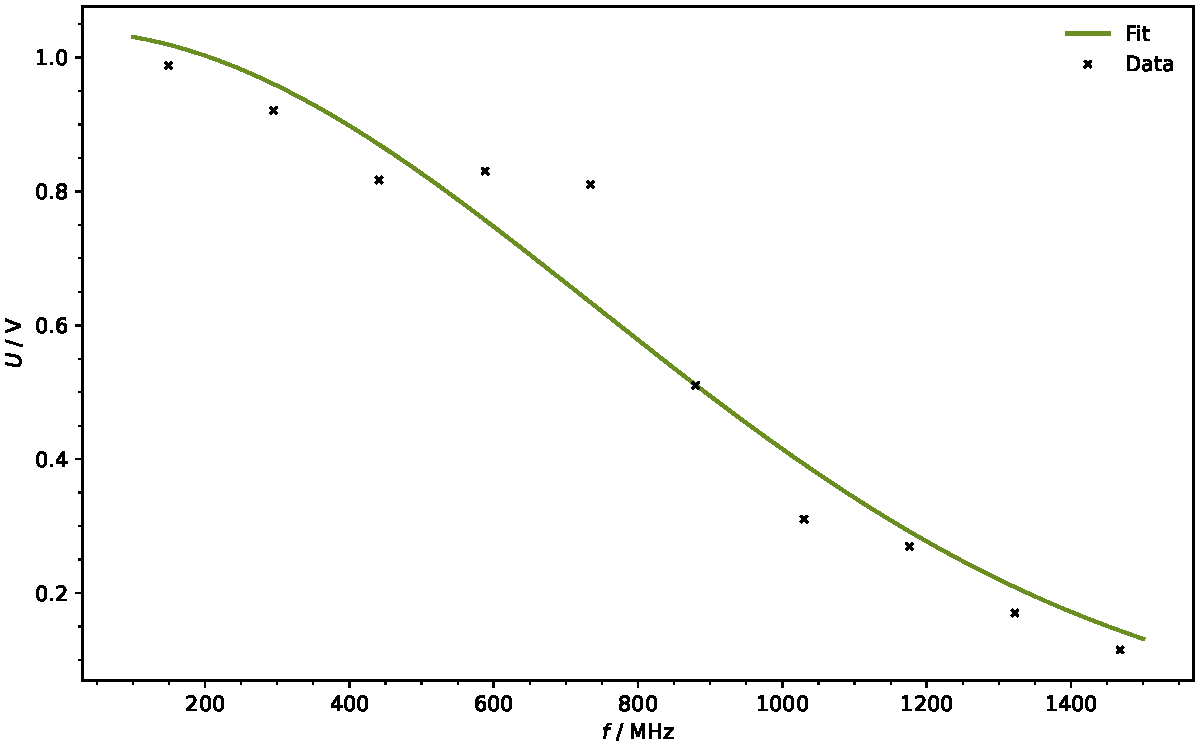
\includegraphics[width=0.8\textwidth]{content/plots/AUA.pdf}
    \caption{Measurement and visualization of Doppler broadening.}
    \label{fig:BRUCH}
\end{figure}
The fitted curve follows the form 
\begin{equation*}
    U(f)= n\cdot \exp\left(-\frac{(f-m)^2}{2s^2}\right)\; .
\end{equation*}

The parameters can be determined to
\begin{align*}
    n &= (1.04 \pm 0.05)\, \text{V} \\
    s &= (738 \pm 43) \, \text{MHz}\; .
\end{align*}
From here the full width half maximum ($\Delta f_{\text{D}}$) can be calculated using \eqref{eqn:fwhm}
\begin{equation*}
    \Delta f_{\text{D}} = (1.7 \pm 0.1) \, \text{GHz}\; . 
\end{equation*}
In comparison, the theoretical value mentioned in \autoref{sec:doppler} is $\Delta f_\text{D} \approx \qty{1.5}{\giga\hertz}$ for a \HeNe laser.
